\documentclass[a4paper,english]{scrreprt}

% Uncomment to optimize for double-sided printing.
% \KOMAoptions{twoside}

% Set binding correction manually, if known.
% \KOMAoptions{BCOR=2cm}

% Localization options
\usepackage[english]{babel}
\usepackage[T1]{fontenc}
\usepackage[utf8]{inputenc}

% Enhanced verbatim sections. We're mainly interested in
% \verbatiminput though.
\usepackage{verbatim}

% PDF-compatible landscape mode.
% Makes PDF viewers show the page rotated by 90°.
\usepackage{pdflscape}

% Advanced tables
\usepackage{tabu}
\usepackage{longtable}
\usepackage{dcolumn}
\newcolumntype{d}[1]{D{.}{\cdot}{#1} }

% Fancy tablerules
\usepackage{booktabs}

% Graphics
\usepackage{graphicx}

% Current time
\usepackage[useregional=numeric]{datetime2}

% Float barriers.
% Automatically add a FloatBarrier to each \section
\usepackage[section]{placeins}

% Custom header and footer
\usepackage{fancyhdr}

\usepackage{geometry}
\usepackage{layout}

% Math tools
\usepackage{mathtools}
% Math symbols
\usepackage{amsmath,amsfonts,amssymb}
\usepackage{amsthm}

% SI units
\usepackage{siunitx}
\DeclareSIUnit\Molar{\textsc{m}}
\DeclareSIUnit\rpm{\textsc{rpm}}

% Chemistry
\usepackage{mhchem}

% Subfigures & captions
\usepackage{subcaption}
\usepackage{wrapfig}

\DeclarePairedDelimiter\abs{\lvert}{\rvert}

\pagestyle{plain}
% \fancyhf{}
% \lhead{}
% \lfoot{}
% \rfoot{}
% 
% Source code & highlighting
\usepackage{listings}

% Convenience commands
\newcommand{\mailsubject}{2027 - Lab course biochemistry 11}
\newcommand{\maillink}[1]{\href{mailto:#1?subject=\mailsubject}
                               {#1}}

% Should use this command wherever the print date is mentioned.
\newcommand{\printdate}{\today}

\subject{2027 - Lab course biochemistry 1}
\title{3 - Real-time quantitative PCR}

\author{Michael Senn \maillink{michael.senn@students.unibe.ch} - 16-126-880 - Group 14}

\date{\printdate}

% Needs to be the last command in the preamble, for one reason or
% another. 
\usepackage{hyperref}


\begin{document}
\maketitle

\chapter{Introduction}

The goal of this experiment was to analyze the role of sialic acid cell
receptors on the internalization of MVM viruses into mouse fibroplasts.

To do this, some cell samples were treated with neuraminidase to cleave those
receptors and subsequently exposed to the MVM virus. Using qPCR the viral DNA
was amplified, and its initial quantity in treated and untreated cells compared.

\chapter{Protocol}

The experiment was done based on the provided protocol \cite{skriptv3}. The
following will list any relevant steps taken by us, including potential
deviations from the protocol.

\section{Sample preparation}

A cell suspension was prepared ahead of time, containing $2.5 \cdot 10^5$ cells
per \SI{180}{\ul}. A dilution of neuraminidase in glycobuffer was created, with
a concentration of \SI{0.5}{U \per \ul}.

Then, four samples were prepared according to the following table.
\\

\begin{tabu}{lllll}
	\toprule
	Sample & N-1 & N-2 & N+1 & N+2 \\
	\midrule
	Cell suspension & \SI{180}{\ul} & \SI{180}{\ul} & \SI{180}{\ul} & \SI{180}{\ul} \\
	Neuraminidase dilution & \SI{0}{\ul} & \SI{0}{\ul} & \SI{20}{\ul} & \SI{20}{\ul} \\
	Glycobuffer & \SI{20}{\ul} & \SI{20}{\ul} & \SI{0}{\ul} & \SI{0}{\ul} \\
	\bottomrule
\end{tabu}
\\

The four samples were mixed on a vortexer, and incubated for \SI{30}{\minute}
at \SI{37}{\celsius}, to facilitate activity of the neuraminidase.

\section{Virus internalisation}

\SI{10}{\ul} of a MVM-infected supernatant, with a concentration of $10^7$
virions per \si{\ul}, were added to all samples. The samples were then mixed on
a vortexer, and incubated for \SI{1}{\hour} at \SI{37}{\celsius}.

\section{Washing the samples}

In order to remove excess virus, the samples were washed thrice. During each
cycle they were first centrifuged at \SI{3000}{g} for \SI{3}{\min}, the
supernatant then discarded and the pellets resuspended in \SI{900}{\ul} ice-cold
PBS. After the final washing cycle, the supernatant was removed.

After the second centrifugation sample N$-$2 was accidentally resuspended in
its supernatant, so had to undergo an additional centrifugation to restore the
pellet and prevent loss of cells.

\section{Lysis with Chelex}

Through rapid pipetting a provided Chelex suspension of \SI{100}{\mg \per \ml}
was homogenized, and \SI{500}{\ul} transferred to a separate tube. This
solution was homogenized once more and \SI{100}{\ul} were added to each
sample. The samples were vortexed and incubated for \SI{10}{\min} at
\SI{95}{\celsius}, while shaking at \SI{400}{\rpm}.

During this step sample N$+$2 accidentally had \SI{400}{\ul} instead of
\SI{100}{\ul} of Chelex added, so a higher dilution is expected.

Afterwards the samples were cooled down to prevent vapor build-up, vortexed
once more, and centrifuged for \SI{1}{\min} at \SI{15000}{\rpm}.

\SI{25}{\ul} of each sample's supernatant, containing the DNA, was added to a
separate tube, to be used in the following qPCR.

\section{Preparation of qPCR master-mix}

Two types of qPRC master-mix were prepared. The first one contained iTaq-mix,
forward primer and reverse primer, the second one was identical except for no
added reverse primer.

Composition of the first master-mix:
\\

\begin{tabu}{lll}
	\toprule
	Component & Fractions & Volume \\
	\midrule
	iTaq mix & 16 & \SI{112}{\ul} \\
	Forward primer MVM-F & 1 & \SI{7}{\ul} \\
	Reverse primer MVM-R-489 & 1 & \SI{7}{\ul} \\
	\bottomrule
\end{tabu}
\\

Composition of the second master-mix:
\\

\begin{tabu}{lll}
	\toprule
	Component & Fractions & Volume \\
	\midrule
	iTaq mix & 16 & \SI{112}{\ul} \\
	Forward primer MVM-F & 1 & \SI{7}{\ul} \\
	\bottomrule
\end{tabu}

\section{Preparation of PCR samples}

\SI{18}{\ul} of the first master-mix were added to five wells. Afterwards the
four samples, plus pure \ce{H2O} as a negative control, were added to these
wells.

\SI{17}{\ul} each of the second master-mix were added to six additional wells.
\SI{1}{\ul} of different reverse primers were added, with MVM-R-72 being added
to wells 6 and 7, MVM-R-432 to wells 8 and 9, and MVM-R-1037 to wells 10 and
11. Afterwards \SI{2}{\ul} of the samples without neuraminidase were added to
those wells, with sample 1 being added to wells 6, 8, 10, and sample 2 being
added to wells 7, 9 and 11.

In summary, the following wells were prepared:
\\

\begin{tabu}{lccccccccccc}
	\toprule
	Well & 1 & 2 & 3 & 4 & 5 & 6 & 7 & 8 & 9 & 10 & 11 \\
	\midrule 
	iTaq Mix & \SI{16}{\ul} & \SI{16}{\ul} & \SI{16}{\ul} & \SI{16}{\ul} & \SI{16}{\ul} & \SI{16}{\ul} & \SI{16}{\ul} & \SI{16}{\ul} & \SI{16}{\ul} & \SI{16}{\ul} & \SI{16}{\ul} \\
	MVM-F & \SI{1}{\ul} & \SI{1}{\ul} & \SI{1}{\ul} & \SI{1}{\ul} & \SI{1}{\ul} & \SI{1}{\ul} & \SI{1}{\ul} & \SI{1}{\ul} & \SI{1}{\ul} & \SI{1}{\ul} & \SI{1}{\ul} \\
	MVM-R-489 & \SI{1}{\ul} & \SI{1}{\ul} & \SI{1}{\ul} & \SI{1}{\ul} & \SI{1}{\ul} &  &  &  &  &  &  \\
	MVM-R-72 & & & & & & \SI{1}{\ul} & \SI{1}{\ul} & & & & \\
	MVM-R-432 & & & & & & & & \SI{1}{\ul} & \SI{1}{\ul} & & \\
	MVM-R-1037 & & & & & & & & & & \SI{1}{\ul} & \SI{1}{\ul} \\
	N$+$ 1 & \SI{2}{\ul} & & & & & & & & & & \\
	N$+$ 2 & & \SI{2}{\ul} & & & & & & & & & \\
	N$-$ 1 & & & \SI{2}{\ul} & & & \SI{2}{\ul} & & \SI{2}{\ul} & & \SI{2}{\ul} & \\
	N$-$ 2 & & & & \SI{2}{\ul} & & & \SI{2}{\ul} & & \SI{2}{\ul} & & \SI{2}{\ul} \\
	\ce{H2O} & & & & & \SI{2}{\ul} & & & & & & \\
	\bottomrule
\end{tabu}
\\

The second group also prepared four wells with known standards, containing
$10^7, 10^6, 10^5$ and $10^4$ plasmides of the MVM genome in the first
master-mix respectively.

\section{qPCR}

The various wells subsequently underwent 40 PCR cycles, optimized for the
reverse primer MVM-R-489, followed by a melting curve analysis.

\begin{itemize}
	\item Hot start, \SI{95}{\celsius}, \SI{5}{\min}
	\item 40 PCR cycles
		\begin{itemize}
			\item Denaturation, \SI{95}{\celsius}, \SI{15}{\s}
			\item Annealing , \SI{61}{\celsius}, \SI{15}{\s}
			\item Extension, \SI{72}{\celsius}, \SI{15}{\s}
		\end{itemize}
	\item End, \SI{95}{\celsius}, \SI{1}{\min}
	\item Melting curve, \SIrange{65}{95}{\celsius}, \SI{10}{\s \per \celsius}
\end{itemize}

During qPCR, fluorescence of the added dye was measured, and stored for
further analysis.

\chapter{Results \& discussion}

\section{qPCR results}

The following starting quantities were calculated as part of the qPCR. N$+$ are
samples with, N$-$ without neuraminidase.

\subsection{Own results}

Figure \ref{fig:sq_14} shows values based on the samples prepared by our group.
\\

\begin{tabu}{lll}
	\toprule
	& N$+$ & N$-$ \\
	\midrule
	Sample 1 & 139884 & 146774 \\
	Sample 2 & 135924 & 428253 \\
	Mean & 137904 & 287514 \\
	Stdev & 2800 & 199035 \\
	\bottomrule
\end{tabu}

\begin{figure}
	\centering
	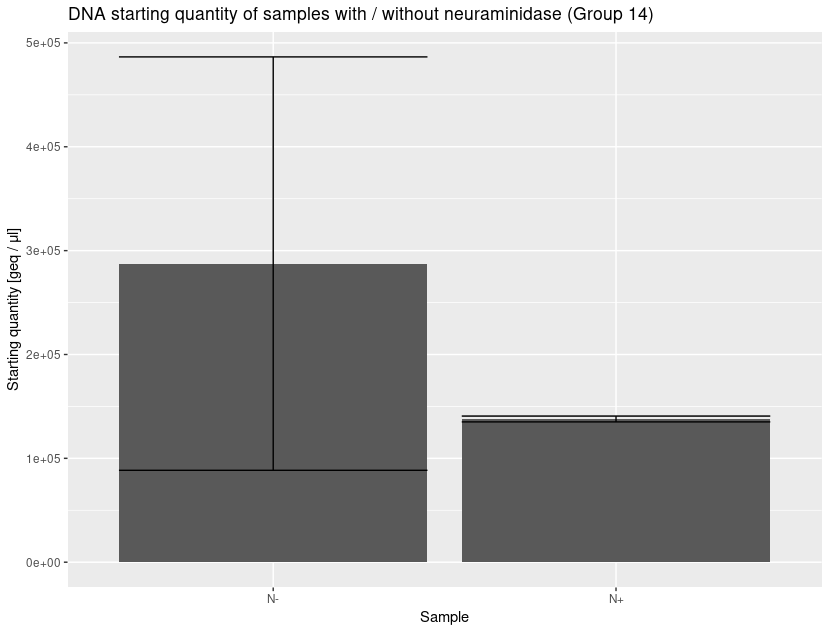
\includegraphics[width=0.8\textwidth]{img/sq_group14.png}
	\caption{Results group 14}
	\label{fig:sq_14}
\end{figure}

\subsection{Results of different group}

Figure \ref{fig:sq_xx} shows values based on the samples prepared by another
group, for the sake of comparison in the following discussion.
\\

\begin{tabu}{lll}
	\toprule
	& N$+$ & N$-$ \\
	\midrule
	Sample 1 & 60200 & 488000 \\
	Sample 2 & 66300 & 630000 \\
	Mean & 63250 &  559000 \\
	Stdev & 4313 & 100409 \\
	\bottomrule
\end{tabu}

\begin{figure}
	\centering
	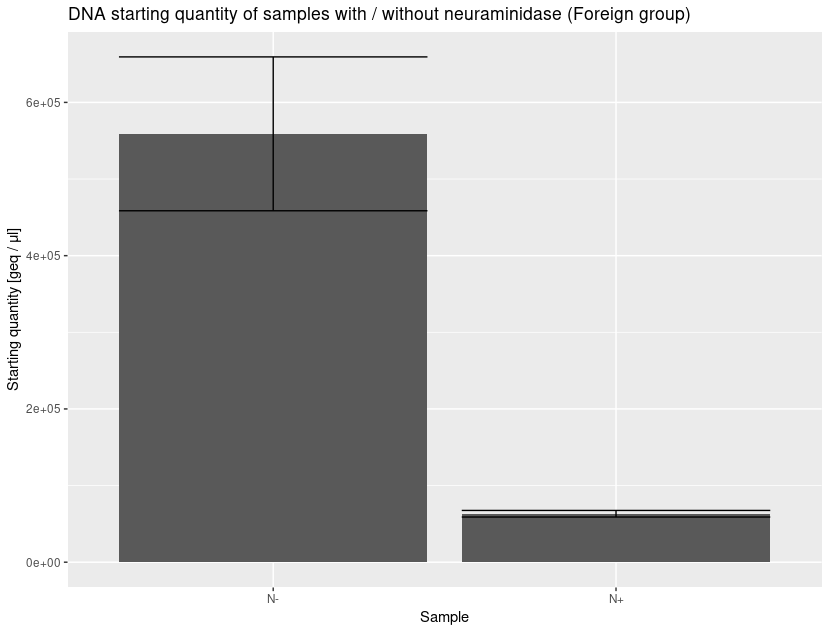
\includegraphics[width=0.8\textwidth]{img/sq_groupxx.png}
	\caption{Results external group}
	\label{fig:sq_xx}
\end{figure}

\subsection{Multiplicity of infection}

Each of our \SI{200}{\ul} samples contained \SI{180}{\ul} cell suspension, with
a concentration of $2.5 \cdot 10^5$ cells per \SI{180}{\ul}. To each we added
\SI{10}{\ul} MVM-infected supernatant, with a concentration of $10^7$ virions
per \si{\ul}.

Hence each sample contains $\SI{10}{\ul} \cdot 10^7 \si{virions \per \ul} =
10^8 \si{virions}$, and $\SI{180}{\ul} \cdot 2.5 \cdot 10^5 \si{cells \per 180 \ul}
= 2.5 \cdot 10^5 \si{cells}$, for a MOI of:

\[
	\text{MOI} = \frac{10^8 \si{virions}}{2.5 \cdot 10^5 \si{cells}} = \SI{400}{virions \per cell}
\]

\section{Expected vs actual qPCR measurements}

The goal of the experiment was to verify that the MVM virus uses sialic acid
as a cell receptor for the purpose of internalisation. As neuraminidase will
cleave the sialic acid groups of cells, we expected treated samples to have a
significantly lower concentration of viral DNA.

\subsection{Viral DNA in untreated samples}

While the measured averages do confirm this, the high standard deviation of the
untreated samples inspires little confidence that this is anything more than
chance. When comparing our results with the external results in figure
\ref{fig:sq_xx}, it becomes clear that the high standard deviation is likely
the result of a mistake, or inaccuracies, in the experiment's execution.

It is possible that not all samples were washed equally well, such that one of
the two had high concentrations of external viruses left over. This would also
fit well with the higher than expected concentration of viral DNA in the
treated sample, where no internalisation should have occurred.

\subsection{Viral DNA in treated samples}

The high concentration of viral DNA in the treated samples might be the result
of the too short incubation time after having added the neuraminidase. Due to
the high number of sialic acid receptors, thirty minutes might not have been
enough to cleave all receptors, allowing some viral DNA to enter the treated
cells.

Interestingly enough there is also no significant difference between the two
treated samples, in spite of N$+$-2 being three times as diluted as N$+$-1.

\section{Matching reverse primer sequences with fragment lengths}

NCBI BLAST \cite{website:blast} was used to find the locations of the forward
and reverse primers in the MVM genome. This lead to the positions shown in
figure \ref{fig:primer_locations}, as well as the following table.
\\

\begin{tabu}{lll}
	\toprule
	Sequence & Start & End \\
	\midrule
	Forward: 5’-TTC ATT CTG TGA GTC GAG ACG CAC-3’ & 214 & 237 \\
	1: 5’-TGC CTT CTC CAC CAT TTC CCT TGA-3’ & 680 & 703 \\
	2: 5’-CAT CAG AGT AAG CAT TTC CAG-3’ & 265 & 285 \\
	3: 5’-ACA AAT CTC TAG CGT ATT TTT-3’ & 1230 & 1250 \\
	4: 5’-CGC AGT GCC AGC CTT GGT CTT TTC-3’ & 622 & 644 \\
	\bottomrule
\end{tabu}
\\

\begin{figure}
	\centering
	\begin{subfigure}{.475\textwidth}
		\centering
		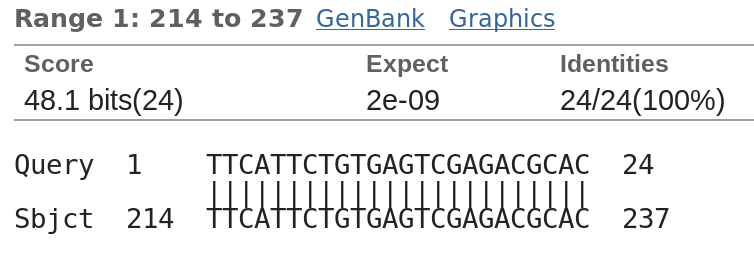
\includegraphics[width=\linewidth]{img/primer_forward.png}
		\caption{Forward primer}
		\label{fig:primer_forward}
	\end{subfigure}%
	\vskip\baselineskip
	\begin{subfigure}{.475\textwidth}
		\centering
		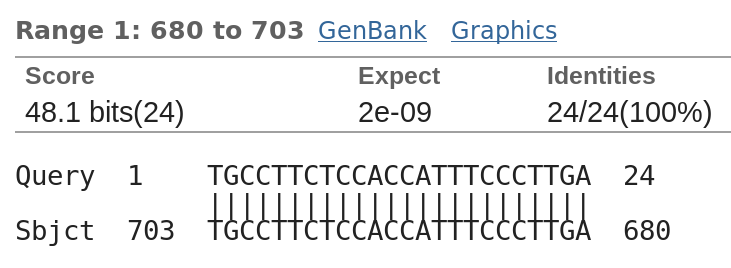
\includegraphics[width=\linewidth]{img/primer_1.png}
		\caption{Reverse primer 1}
		\label{fig:primer_1}
	\end{subfigure}%
	\begin{subfigure}{.475\textwidth}
		\centering
		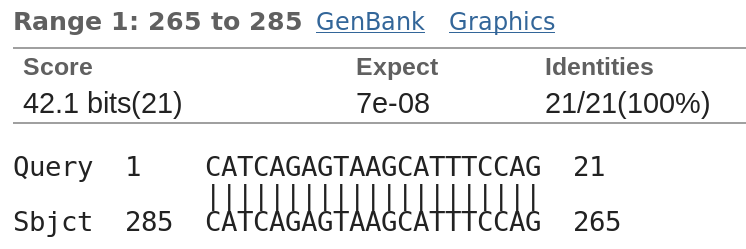
\includegraphics[width=\linewidth]{img/primer_2.png}
		\caption{Reverse primer 2}
		\label{fig:primer_2}
	\end{subfigure}
	\vskip\baselineskip
	\begin{subfigure}{.475\textwidth}
		\centering
		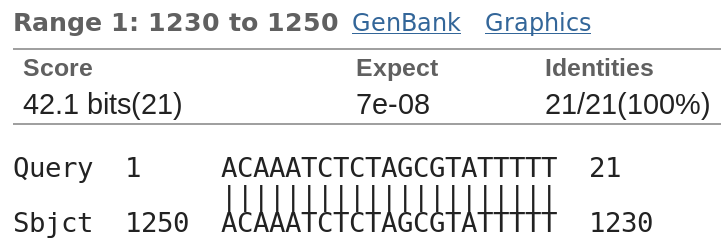
\includegraphics[width=\linewidth]{img/primer_3.png}
		\caption{Reverse primer 3}
		\label{fig:primer_3}
	\end{subfigure}%
	\begin{subfigure}{.475\textwidth}
		\centering
		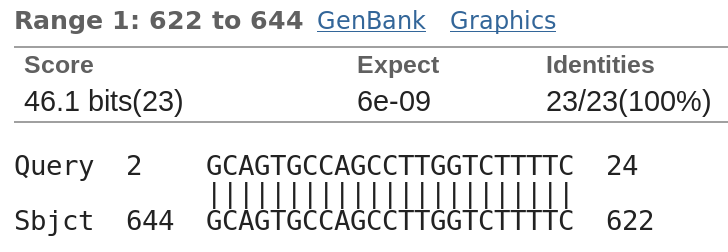
\includegraphics[width=\linewidth]{img/primer_4.png}
		\caption{Reverse primer 4}
		\label{fig:primer_4}
	\end{subfigure}
	\caption{Location of primers in MVM genome}
	\label{fig:primer_locations}
\end{figure}

Noteworthy is that for sequence 4 only 23 of the 24 nucleotides matched, with
the first C not being part of the MVM genome. This might be a typo in the
protocol, or a primer which does not fit perfectly.

Ordering them by position in the genome in ascending order, and calculating the
length of the fragment - starting at the beginning of the forward primer and
ending at the end of the reverse primer, allows associating the reverse primer
sequences 1 through 4 with the used reverse primers:
\\

\begin{tabu}{lll}
	\toprule
	Reverse primer & Sequence number & Fragment length \\
	\midrule
	MVM-R-72 & 2 & $285 - 214 + 1 = 72$ \\
	MVM-R-432 & 4 & $644 - 214 + 1 = 431$ \\
	MVM-R-489 & 1 & $703 - 214 + 1 = 490$ \\
	MVM-R-1037 & 3 & $1250 - 214 + 1 = 1037$ \\
	\bottomrule
\end{tabu}
\\

\section{Primer comparison}

\subsection{Melting curves}

As the melting temperature of a replicated fragment - that is the temperature
at which the double-strand splits into two single strands - depends on the
strength of the non-covalent bonds within the fragment, bigger fragments - with
more non-covalent bonds - are expected to have a higher melt point.

This is visible in figure \ref{fig:melting_curves}, where the melt points are
in ascending order of fragment length, with fragments synthesized with the
MVM-R-72 primer melting first, followed by MVM-R-432, MVM-R-489 and lastly
MVM-R-1037.

It is visible that the effect is not linear, with fragments melting, no matter
their length, once temperature reaches \SI{85}{\celsius}.

\subsection{Amplification}

In figure \ref{fig:amplification} DNA amplification over time for the various
primers is shown. As the utilized PCR was optimized for MVM-R-489, these
samples were expected to be amplified the fastest, and plateau at the highest
level, which is clearly visible in the graph.

The next fastest amplification was of samples with MVM-R-72. This is likely due
to those fragments' small size, allowing them to be amplified with decent speed
even under non-optimal conditions. After that MVM-R-1037 follows, whose
fragments were likely too long to reliably extend during the utilized cycle
times, and whose amplification was so hindered.

Of interest are fragments produced with the reverse primer MVM-R-432, which
seem to have been significantly less amplified than the others. While
amplification levels less than those of MVM-R-489 are to be expected, they
should have been amplified more heavily than those samples with MVM-R-1037 due
to their smaller size.

One theory is that the fluorescent dye is not able to bind to the produced
fragments all too well, such that, even if a lot of fragments are produced,
only few are measured. This is not very convincing however, as the fragments
produced with MVM-R-489 seem to bind the dye well, and have a lot of overlap
with the ones of MVM-R-432.

\begin{figure}
	\centering
	\includegraphics[width=0.9\textwidth]{img/melting_curves.png}
	\caption{Melting curves}
	\label{fig:melting_curves}
\end{figure}

\begin{figure}
	\centering
	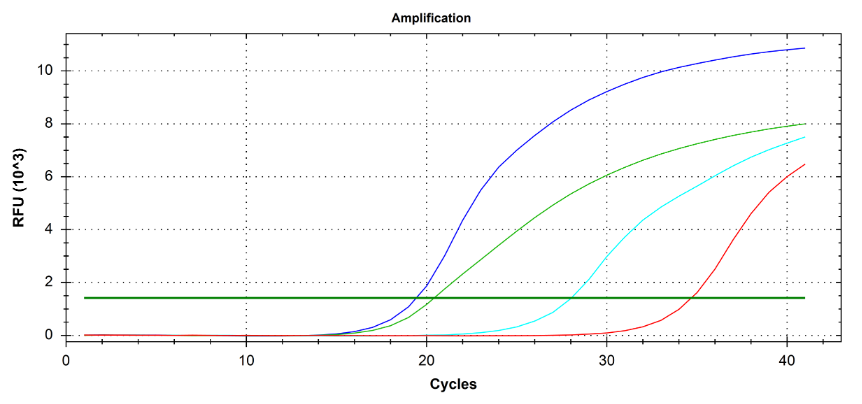
\includegraphics[width=0.9\textwidth]{img/amplification.png}
	\caption{Amplification}
	\label{fig:amplification}
\end{figure}


\bibliographystyle{plainnat}
\bibliography{references}

\end{document}
